\pdfoutput=1

\documentclass[11pt]{article}

\usepackage[final]{final}
\usepackage{times}
\usepackage{latexsym}
\usepackage[T1]{fontenc}
\usepackage[utf8]{inputenc}
\usepackage{microtype}
% \usepackage{inconsolata}
\usepackage{graphicx}
\title{Efficient Image Compression}

\author{James Camacho \\
  MIT / AI \\
  \texttt{jamesc03@mit.edu} \\\And
  Linda He \\
  Harvard / Applied Mathematics \\
  \texttt{lindahe@college.harvard.edu} \\}

\begin{document}
\maketitle
\begin{abstract}
  With high-dimensional spaces such as images or video, perfect communication becomes prohibitively expensive. A lossy, compressed version is cheaper to transmit and often good enough for most purposes. Traditional algorithms such as JPEG use a Fourier transform to pick out the most important features for transmission. In this paper, we explore using auto- and raster-encoders to automatically and efficiently compress images instead. We find they significantly outperform JPEG on the MNIST dataset, and discuss potential future improvements to their speed and cost via reinforcement learning.
\end{abstract}


\section{Introduction}

% TODO: Needs a lot of work.

Over 75\% of internet traffic comes in the form of video \citep{cisco-2018-traffic}, and YouTube alone nets \$30bn from their distribution \citep{alphabet-2024-earnings}. At these massive scales, every extra bit of compression is important. In this paper, we explore more optimal compression with the use of deep learning methods, including one adapted from language models.

Image and text have often been treated as separate domains, but there is much that can be applied between the two. Inspired by quantization and fractalization from image compression, Witten \textit{et al.} proposed several lossy text encoding schemes as far back as 1992 \citep{witten-etal-1992-lossy}. Recent advances in image generation such as denoising models \citep{ho-2020-denoising} have similarly found applications in text generation by interpreting language tokens as pixels \citep{kou-2024-cllms}. Going the other direction, the popular Transformer architecture of language models have been applied to vision \citep{dosovitskiy-2021-vit}, and has seen state-of-the-art success in video production \citep{liu-2024-sora}.

The Vision Transformer algorithm bears a striking resemblance to JPEG, and this is no coincidence. Generation is the inverse of compression, and more generally ``being able to compress well is closely related to acting intelligently'' \citep{hutter-2020}. Unfortunately, this enforces a tradeoff between the algorithm's speed and size. For example, an unintelligent compressor may store images verbatim, or a generator may simply sample from its training dataset. Smarter algorithms will do much better, but require more computation.

This paper will focus on the tradeoff between image quality and compression length, but we will end with several suggestions for improving the running time via reinforcement learning.


\section{Related Work}

\section{Data}

MNIST, separate train and test sets.

\section{Methods}

\subsection{JPEG}\label{sec:jpeg}

These vision transformers bear a striking resemblance to the JPEG algorithm

\subsection{Auto-Encoders}

\begin{figure*}[t]
  \centering
  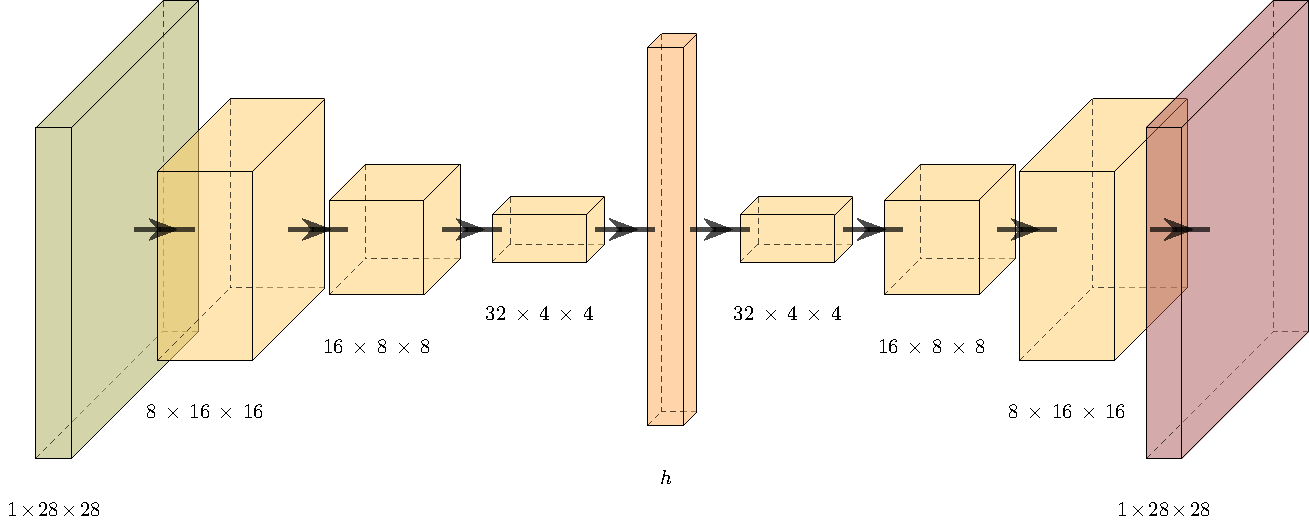
\includegraphics[width=2\columnwidth]{diagrams/auto.pdf}
  \caption{Auto-encoder network.}
  \label{fig:auto}
\end{figure*}

\begin{figure*}[t]
  \centering
  
\includegraphics[width=0.2\columnwidth]{diagrams/reconstructions/original.png}
  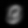
\includegraphics[width=0.2\columnwidth]{diagrams/reconstructions/0.png}
  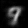
\includegraphics[width=0.2\columnwidth]{diagrams/reconstructions/1.png}
  
\includegraphics[width=0.2\columnwidth]{diagrams/reconstructions/2.png}
  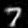
\includegraphics[width=0.2\columnwidth]{diagrams/reconstructions/4.png}
  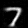
\includegraphics[width=0.2\columnwidth]{diagrams/reconstructions/8.png}
  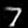
\includegraphics[width=0.2\columnwidth]{diagrams/reconstructions/16.png}
  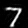
\includegraphics[width=0.2\columnwidth]{diagrams/reconstructions/32.png}
  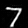
\includegraphics[width=0.2\columnwidth]{diagrams/reconstructions/64.png}
  \caption{Reconstructions of a sample image (left). To the right, $h=0, 1, 2, 4, 8, 16, 32, 64$.}
  \label{fig:recon}
\end{figure*}

Auto-encoders consist of an encoder and a decoder network trained together. Our encoder consists of three convolutional layers and a linear layer to control the latent dimension $h$, and the decoder has the reverse process (see Figure \ref{fig:auto}). By default, PyTorch stores floats using four bytes, so the encoding length takes $4h$ bytes.

To train, we use the mean-squared error between the original and decoded images, running through two epochs of the MNIST training set with the Adam optimizer at $\gamma=10^{-3}$. We keep a separate dataset for testing. Sample reconstructions can be seen in Figure \ref{fig:recon}. As expected, the quality improves as the latent dimension increases, though they remain blurry. This is an artifact of our loss function. Minimizing the squared error,

$$L_2 = \sum (x-\mathrm{correct})^2$$

is equivalent to maximizing the log-likelihood under a Gaussian prior for the error function:

$$L_2 = \log\prod e^{(x-\mathrm{correct})^2}.$$

The actual distribution of error is decidedly not Gaussian, so this biases the reconstruction towards a higher entropy than necessary. A common fix is to add a small adversarial loss \citep{makhzani-2016-adversarial}, but since our quality metric is the $L_2$ loss, we opt to keep the bias. We will use this bias to improve our raster-encoder.

\begin{figure}[h]
  \centering
  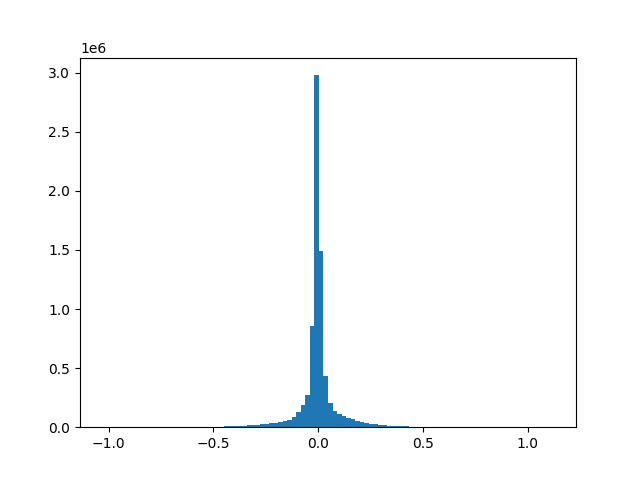
\includegraphics[width=\columnwidth]{diagrams/hist.png}
  \caption{Error hisogram, 100 bins.}
  \label{fig:hist}
\end{figure}

\subsection{Raster-Encoders}

\begin{figure*}[t]
  \centering
  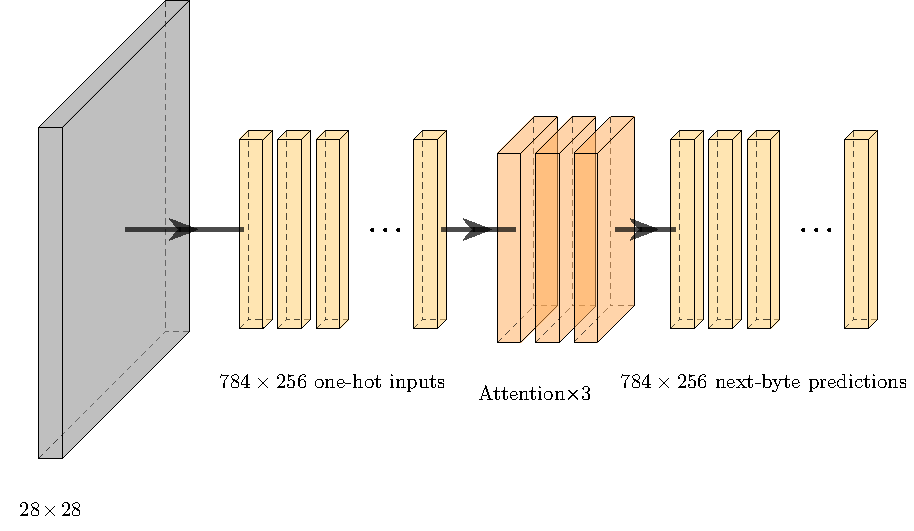
\includegraphics[width=2\columnwidth]{diagrams/raster.pdf}
  \caption{Raster-encoder network.}
  \label{fig:raster}
\end{figure*}



\section{Results}


\section{Discussion}

Testing this: This is some text with a citation \citep{lazaridou-etal-2020-multi}.

\section*{Acknowledgments}

\bibliography{references}

\appendix

\section{Example Appendix}
\label{sec:appendix}

This is an appendix.

\end{document}
